\chapter{Additional Considerations Regarding FSRS Signals from Semiconductor Nanocrystals}    % First appendix chapter, i.e., Appendix A.

\section{FSRS gain at Stokes and anti-Stokes Frequencies}     % This is appendix section 1.
Atypically, the CdSe phonon features exhibit gain at both Stokes and anti-Stokes frequencies, however, such an observation is not unprecedented. In the report of a FSRS study of rhodamine 6G (R6G), Frontiera \emph{et al.} describe a progression from negative to positive anti-Stokes features as the Raman pump wavelength became increasingly more resonant with R6G’s primary absorption feature \cite{DzhaganPhonon, frontiera2008origin}. The authors attributed anti-Stokes Raman gain to Raman processes which are initiated by an interaction with the probe pulse; such processes are enhanced by overlap of the probe pulse and sample absorption spectrum. In light of this, it is possible that the inhomogeneously broadened CdSe NC absorption spectrum (Fig. \ref{f:fsrs1}, inset) provides a quasi-continuum of resonant transitions that can absorb probe photons, thereby enhancing the contribution of probe-initiated scattering pathways such as inverse Raman scattering and hot luminescence. In contrast to Frontiera \emph{et al.}, we observe little dependence of the LO phonon lineshape on Raman pump frequency, as shown below in Figure \ref{f:fsrssup1}. This is also likely due to the broad absorption spectrum of CdSe NCs as compared to R6G. Figure \ref{f:fsrs2}(a) in the main manuscript also shows a broad featureless background arising from hot luminescence pathways. The inset in Figure \ref{f:fsrs2}(a) displays the background-subtracted anti-Stokes 1LO phonon peak. 

\begin{figure}
\begin{center}
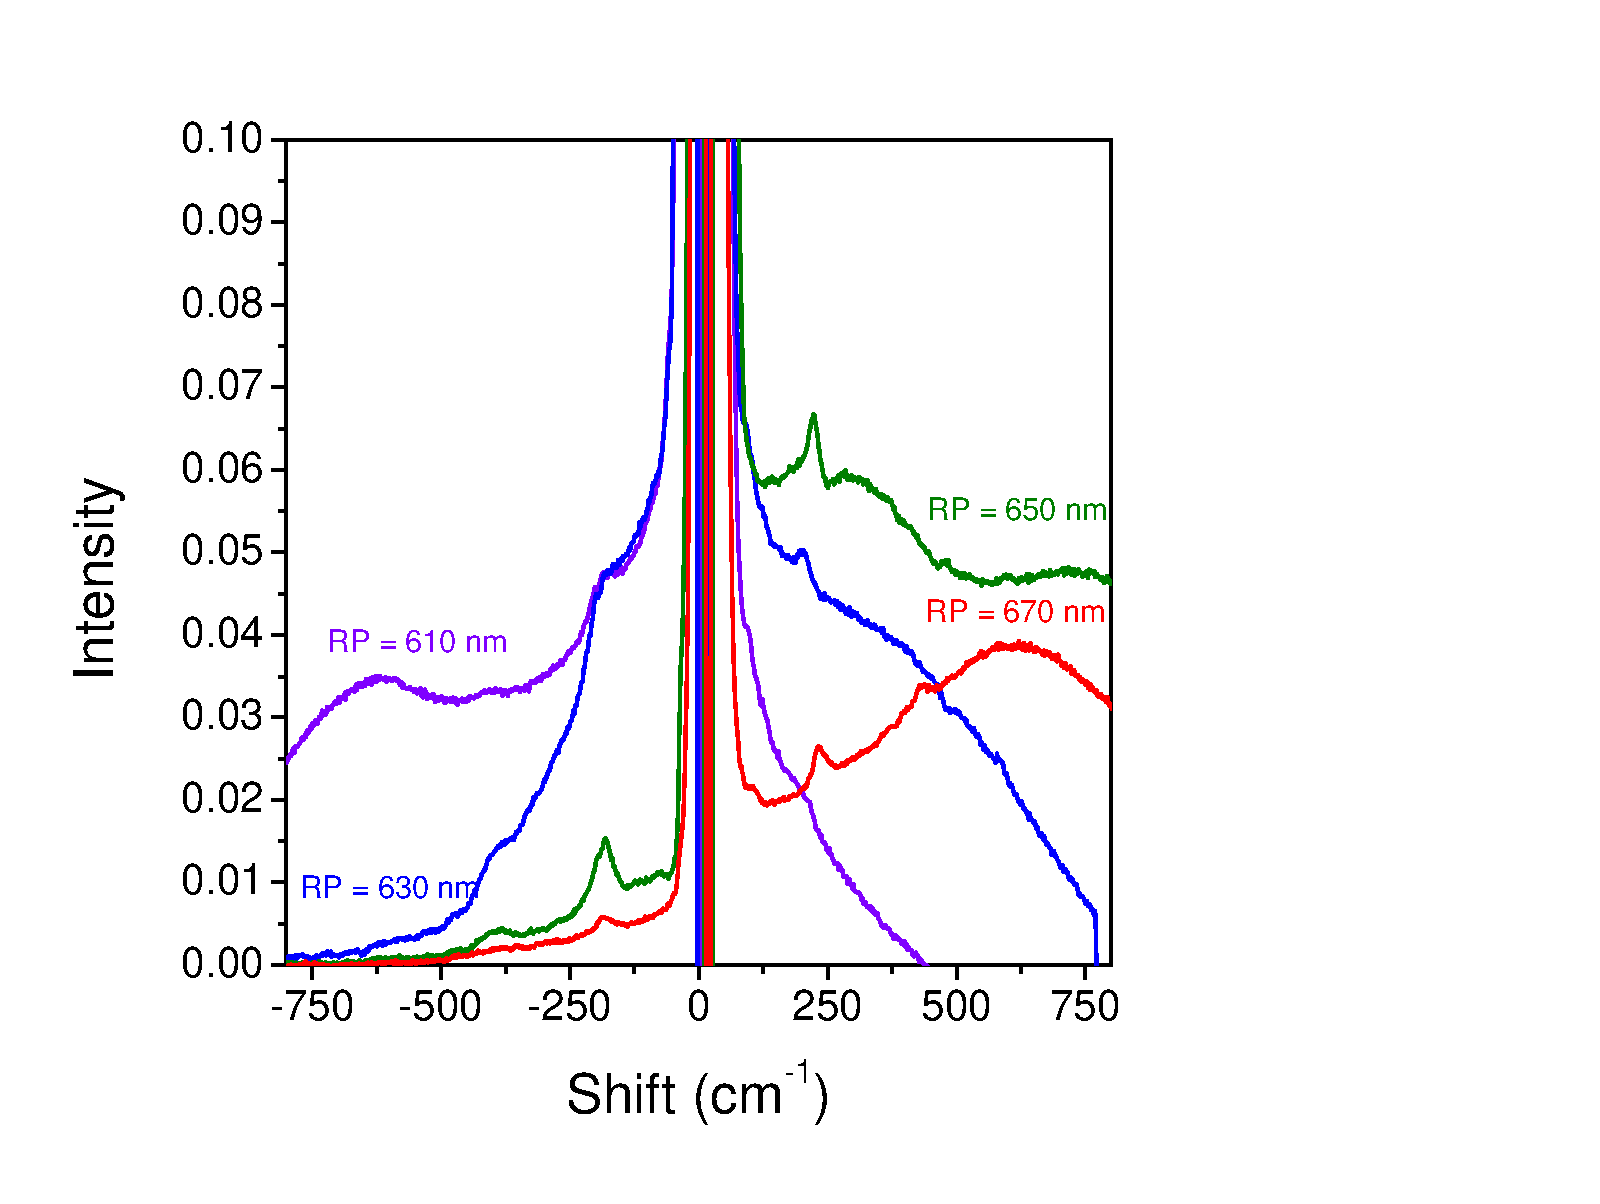
\includegraphics[width=\textwidth]{./appendixB/fsrssup1.pdf}
\caption[Ground state FSRS spectrum of CdSe NCs at a variety of pump wavelengths.]{Raw, ground-state FSRS spectrum for 2.4 nm-diameter CdSe NCs at various Raman pump ("RP") wavelengths, indicated and color-coded in the figure panel.}
\label{f:fsrssup1}
\end{center}
\end{figure}

\section{Impact of Electrostriction on LO Phonon Frequency Shifts} 
In Chapter 2, we note transient softening of the CdSe longitudinal-optical (LO) phonon mode and attribute it to exciton-phonon coupling. However, we cannot exclude, \emph{a priori}, the possibility of changes in phonon frequency due to an electrostriction effect similar to that observed by Wen \emph{et al.} \cite{wen2013electronic}. Specifically, Wen and co-workers observed an ultrafast photoinduced change in strain arising from charge carrier migration to opposite sides of a bismuth ferrous oxide (BFO) thin film. This charge separation subjects the BFO thin film to a changing electric field, resulting in a change of electrostriction. Therefore, in this appendix, we estimate the magnitude and energetics of such an effect for the case of small ($R < 3$ nm), spherical CdSe nanocrystals having a wurtzite crystal structure. We conclude that the changes in phonon frequency observed in our experiments are not consistent with electrostrictive effects both by the sign or magnitude of the predicted interaction. Following the formalism of Wen \emph{et al.} \cite{wen2013electronic}, the strain and peak electric field are related to each other \emph{via} the piezoelectric coefficient as shown in Equation \ref{eq:fsrssup1}:
\begin{equation}\label{eq:fsrssup1}
\sigma_{ij}d_{ij} = |E|
\end{equation}
In Equation \ref{eq:fsrssup1}, $\sigma_{ij}$ is the strain along the axis $ij$ and $d_{ij}$ is the related piezoelectric coefficient. For the wurtzite crystal structure, there are 3 unique axes with piezoelectric coefficients of $d_{15} = -10.51$, $d_{13} = -3.92$, and $d_{33} = 7.84$ pm/V \cite{adachi2009properties}. The peak electric experienced by a CdSe nanocrystal of this size containing a single electron-hole pair (consistent with the excitation fluence utilized in our experiments) is not expected to exceed 16.7 kV/cm \cite{billaud2009stark}. Taking this maximum value as an isotropic field applied to the crystal, the expected strain may be computed using Eq. \ref{eq:fsrssup1} to yield strain values of $\sigma_{15} = -1.76 \times 10^{-5}$, $\sigma_{13} = -0.65 \times 10^{-5}$, and $\sigma_{33} = 1.31 \times 10^{-5}$. We approximate the hydrostatic strain experienced by the nanocrystal as the sum of the unique strain components:
\begin{equation}\label{eq:fsrssup2}
\sigma = \sum_{ij} \sigma_{ij}
\end{equation}
Making the further approximation that the hydrostatic strain is equal to the longitudinal strain, we can compute the expected change in LO phonon frequency due to the presence of a strain-induced electric field. This shift in phonon frequency ($\Delta\omega_{LO}$) is given by Equation \ref{eq:fsrssup3}:
\begin{equation}\label{eq:fsrssup3}
\Delta\omega_{LO} = \left[\frac{p + 2q}{3\omega_0^2} \cdot \frac{S_{11} + 2S_{12}}{S_{11} + S_{12}} + \frac{\frac{2}{3}\left(q - p\right)}{2\omega_0^2} \cdot \frac{S_{11} - S_{12}}{S_{11} + S_{12}}\right] \cdot \omega_0 \cdot \sigma
\end{equation}
In Equation \ref{eq:fsrssup3}, $p$ and $q$ are phonon deformation potentials, which can be realistically estimated as $-\omega_0^2$ and $-2\omega_0^2$, respectively. $S_{11}$ and $S_{12}$ are compliance tensor elements, while $\omega_0$ is the unstrained LO phonon frequency ($\hbar\omega_0 = 212$ cm$^{-1}$ for CdSe). The expected shift in LO phonon frequency, using these parameters and strains, is given for a range of compliance tensor values in Figure \ref{f:fsrssup2}: \par

\begin{figure}
\begin{center}
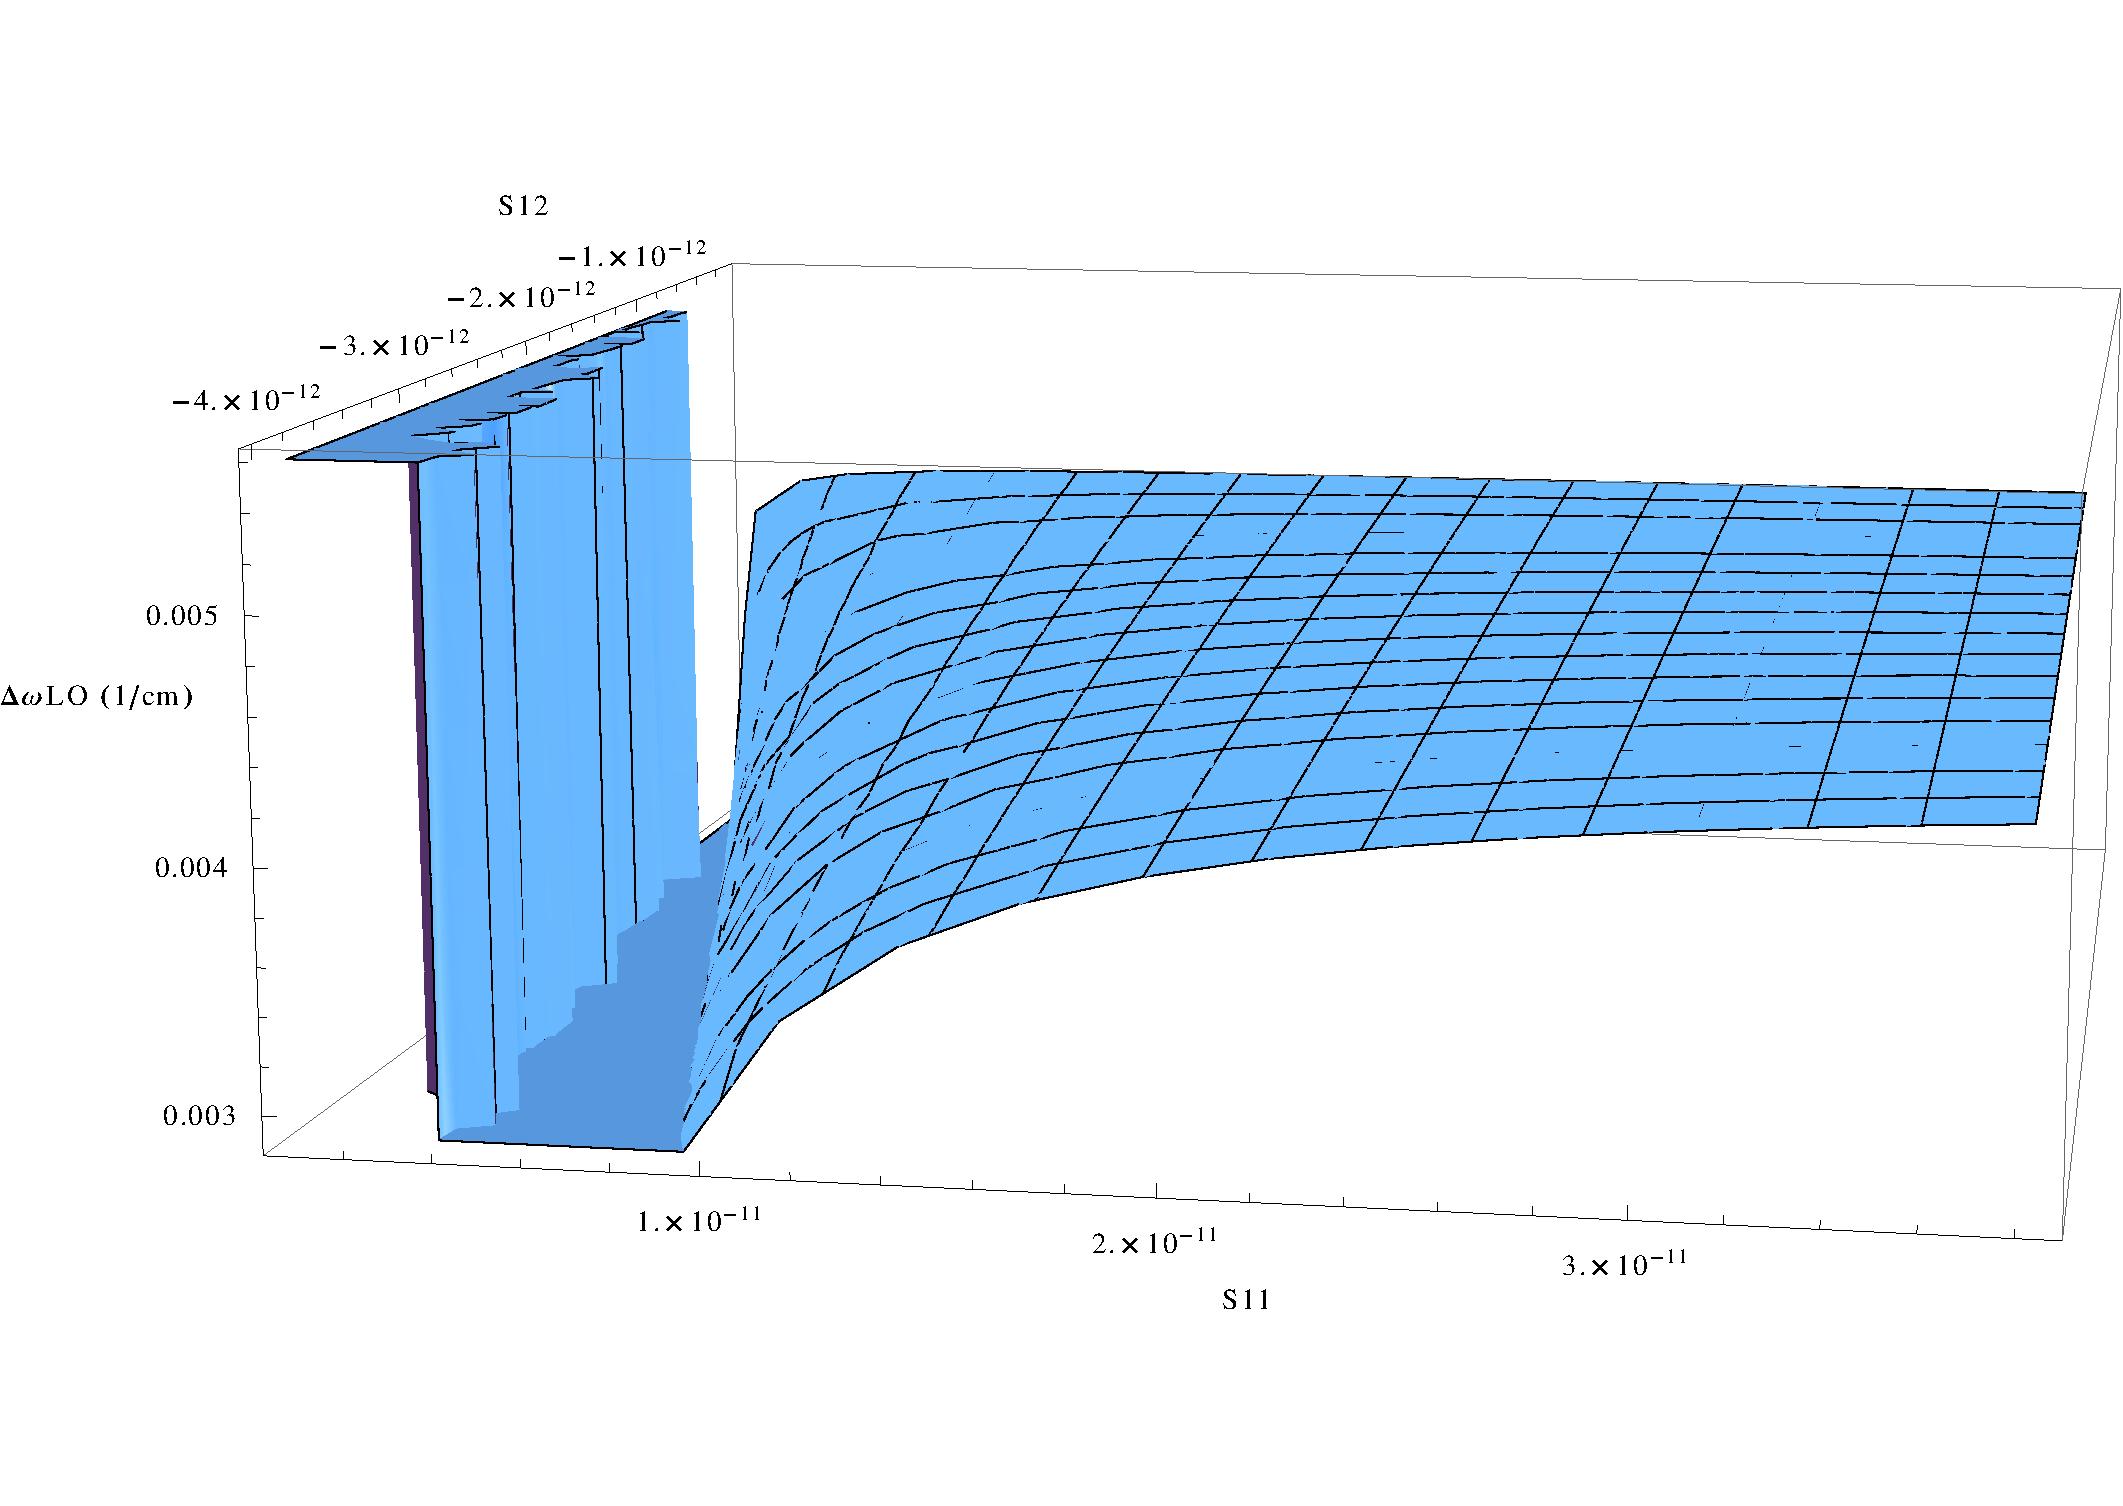
\includegraphics[width=\textwidth]{./appendixB/fsrssup2.pdf}
\caption[Expected electrostriction-induced shift of the LO phonon frequency in CdSe for a range of compliance tensor values.]{Electrostriction-induced shift of the LO phonon frequency ($\Delta\omega_{LO}$) as a function of the compliance tensor elements $S_{11}$ and $S_{12}$. The frequency shift was computed using Eq. \ref{eq:fsrssup3}, the strains given in the text of the Appendix, and an LO phonon energy of 212 cm$^{-1}$.}
\label{f:fsrssup2}
\end{center}
\end{figure}

Although the exact values of the compliance tensor elements for CdSe do not appear to be known at the time of this writing, the range of values plotted in Figure \ref{f:fsrssup2} span an extremely wide range of materials including the potassium halides, silicon, germanium, and diamond carbon \cite{martienssen2006springer}. The mechanical properties of CdSe likely fall somewhere within this (considerable) range. \par

The calculation results shown in Figure \ref{f:fsrssup2} yields two important results. First, in contrast to our experimental observations presented in the main manuscript (a transient red-shift of LO phonon frequency), electric-field induced strain considerations would be expected to increase the LO phonon frequency ($\Delta\omega_{LO} > 0$). This notion of a phonon frequency blueshift with increasing lattice strain is supported by previous works that have found the LO phonon peak in CdS to increase in frequency with increasing hydrostatic pressure \cite{lewis2001handbook}. \par

Secondly, the predicted magnitude of an electric-field induced shift is extremely small ($\sim$0.005 cm$^{-1}$) for the range of compliance tensor elements studied. By contrast, the shift observed in our presented data for the LO phonon frequency is several orders of magnitude larger, on the order of $\sim$2 cm$^{-1}$. Repeating this calculation under the assumptions that electrons and holes are localized and separated by the NC diameter (a physically unlikely scenario), we find a peak electric field that is $\sim$10 times larger than the one reported here. In this case, the electric field induced shift still remains much smaller than our observed shift, and remains in the opposite energetic direction.

\section{Spontaneous Resonant Raman}
The features observed in our femtosecond stimulated Raman scattering spectra are consistent with previous reports of Raman scattering from CdSe NCs, showing a longitudinal-optical (LO) phonon peak at $\sim$220 cmi$^{-1}$ and corresponding overtones. Figure \ref{f:fsrssup3} shows a spontaneous Raman scattering spectrum collected using a 635-nm source to photoexcite 3.1 nm-radius CdSe NCs.

\begin{figure}
\begin{center}
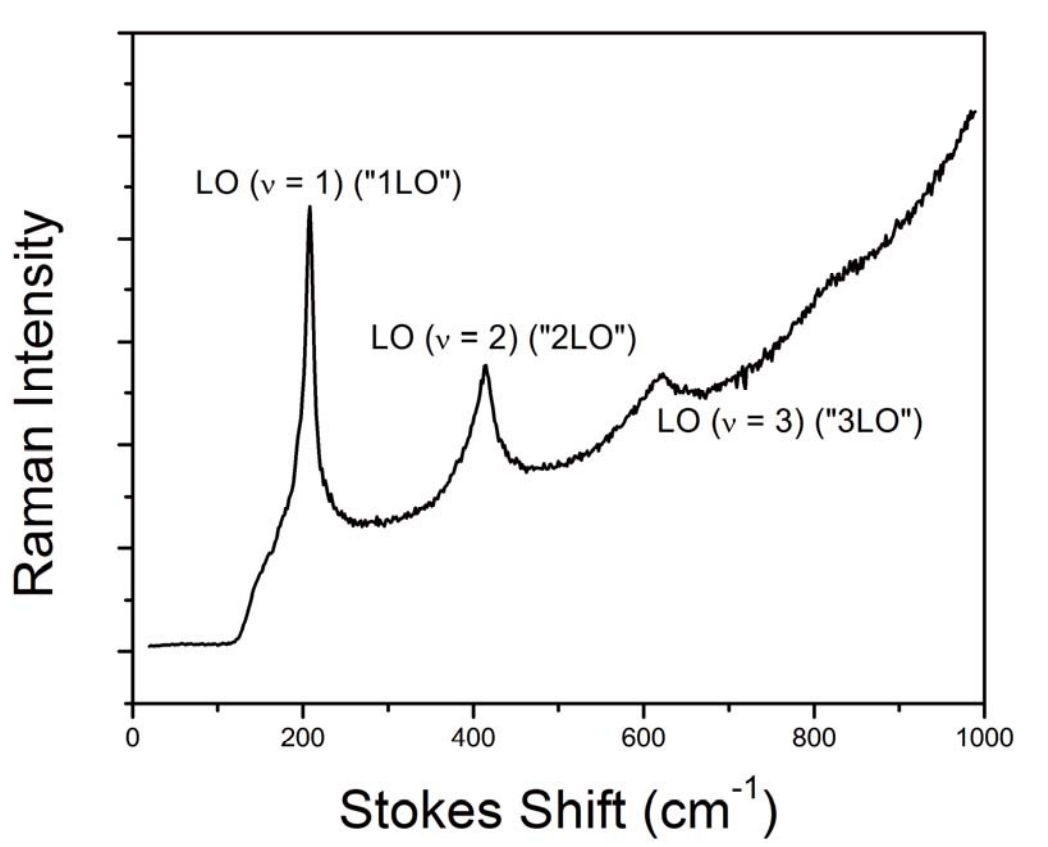
\includegraphics[width=0.65\textwidth]{./appendixB/fsrssup3.png}
\caption[Resonant spontaneous Raman scattering from CdSe NCs.]{Spontaneous Raman spectrum of 3.1 nm-diameter CdSe NCs suspended in hexane. A 635-nm excitation source was used.}
\label{f:fsrssup3}
\end{center}
\end{figure}

\section{Early-time Redshift of LO Phonon Frequency For Additional Nanocrystal Sizes}
It is worth noting that the reported early-time redshift of the CdSe LO phonon feature is observed for both the Stokes and anti-Stokes peaks and occurs for each NC size studied. The red-shifts of the Stokes LO-phonon peak for three sizes of CdSe NC considered in this report are shown in Figure \ref{f:fsrssup4}.

\begin{figure}
\begin{center}
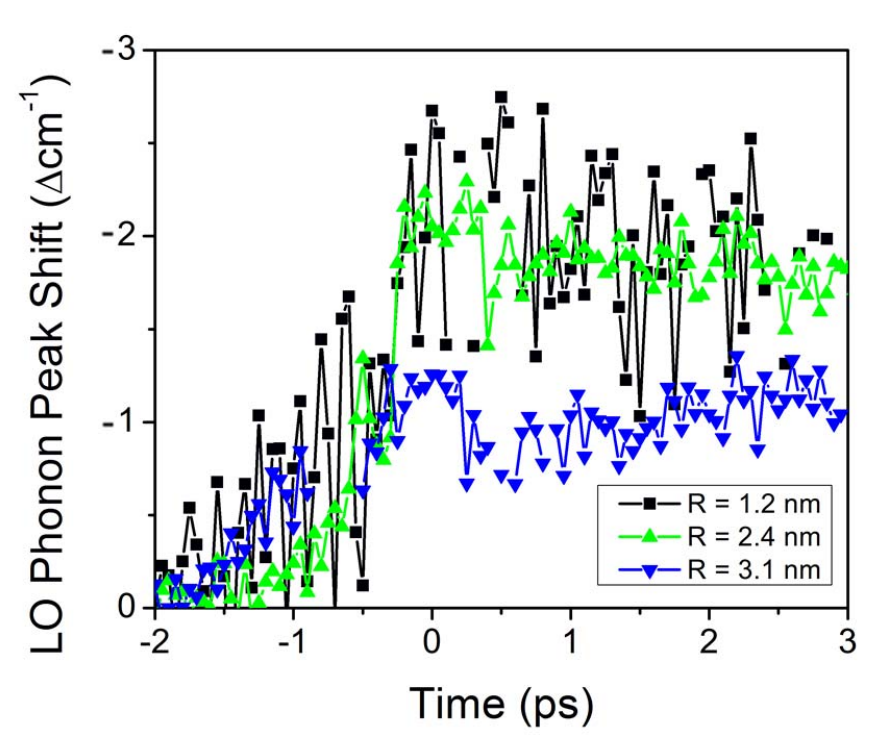
\includegraphics[width=0.65\textwidth]{./appendixB/fsrssup4.png}
\caption[Transient LO phonon softening for a variety of CdSe NC sizes.]{Shift in Stokes LO phonon frequency observed experimentally by FSRS for 3 sizes of CdSe NC. The LO phonon peak center prior to photoexcitation is -221 cm$^{-1}$.}
\label{f:fsrssup4}
\end{center}
\end{figure}

